\chapter{Approach and Implementation}
\label{ch:approach}
%%%%%%%%%%%%%%%%%%%%%%%%%%%%%%%%%%%%%%%%%%%%%%%%%%%%%%%%%%%%%%%%%%%%%%%%%%%%%%%
%%%%%%%%%%%%%%%%%%%%%%%%%%%%%%%%%%%%%%%%%%%%%%%%%%%%%%%%%%%%%%%%%%%%%%%%%%%%%%%
%%%%%%%%%%%%%%%%%%%%%%%%%%%%%%%%%%%%%%%%%%%%%%%%%%%%%%%%%%%%%%%%%%%%%%%%%%%%%%%
%%%%%%%%%%%%%%%%%%%%%%%%%%%%%%%%%%%%%%%%%%%%%%%%%%%%%%%%%%%%%%%%%%%%%%%%%%%%%%%

This chapter describes the basic workflow. The process is mainly driven by an exploratory data analysis approach but primarily follows  Farine's and Whitehead's~\cite{farine2015constructing} steps and key considerations for social network analysis to non-human animal data. Figure~\ref{fig:process} visualizes the adapted and resulting process.

The data set was first analyzed regarding data quality and to form an understanding of the dataset and the behavior of bees in general. Those findings were used to define nodes and infer associations to build the network, respectively derive the parameters for the network pipeline. The resulting networks are analyzed using network science tools and methods. For testing underlying hypothesis the networks are attributed with the bees spatial information and their age. The following sections explain each step in detail.


\begin{figure}[htb]
	\centering
	\includegraphics[width=0.8\textwidth]{Figures/process}
	\caption[Steps of the research approach]{\textbf{Steps of the research approach} [TODO: anpassen, iterationen, hypothesis raus, evtl. so viele Schritte im Bild wie Abschitte im Text, zumindest muss das irgendwie anders.]}
	\label{fig:process}
\end{figure}

\begin{figure}[htb]
	\centering
	\includegraphics[width=1\textwidth]{Figures/setupCams}
	\caption[Camera setup]{\textbf{Camera setup} [Hive=honeycomb, symbol exit as in results, colorscheme]}
	\label{fig:cams}
\end{figure}

%%%%%%%%%%%%%%%%%%%%%%%%%%%%%%%%%%%%%%%%%%%%%%%%%%%%%%%%%%%%%%%%%%%%%%%%%%%%%%%
%%%%%%%%%%%%%%%%%%%%%%%%%%%%%%%%%%%%%%%%%%%%%%%%%%%%%%%%%%%%%%%%%%%%%%%%%%%%%%%
%%%%%%%%%%%%%%%%%%%%%%%%%%%%%%%%%%%%%%%%%%%%%%%%%%%%%%%%%%%%%%%%%%%%%%%%%%%%%%%
%%%%%%%%%%%%%%%%%%%%%%%%%%%%%%%%%%%%%%%%%%%%%%%%%%%%%%%%%%%%%%%%%%%%%%%%%%%%%%%
\section{The Dataset}
\label{sec:dataset}
%%%%%%%%%%%%%%%%%%%%%%%%%%%%%%%%%%%%%%%%%%%%%%%%%%%%%%%%%%%%%%%%%%%%%%%%%%%%%%%
%%%%%%%%%%%%%%%%%%%%%%%%%%%%%%%%%%%%%%%%%%%%%%%%%%%%%%%%%%%%%%%%%%%%%%%%%%%%%%%
%%%%%%%%%%%%%%%%%%%%%%%%%%%%%%%%%%%%%%%%%%%%%%%%%%%%%%%%%%%%%%%%%%%%%%%%%%%%%%%
%%%%%%%%%%%%%%%%%%%%%%%%%%%%%%%%%%%%%%%%%%%%%%%%%%%%%%%%%%%%%%%%%%%%%%%%%%%%%%%

The dataset derives from video files, that capture tagged honey bees of one colony in an observation hive.
The individuals of the colony, including about 3200 bees over a nine weeks period, were tagged with circular 12-bit markers (figure~\ref{fig:markers}, section~\ref{ch:intro}).
Two cameras per side filmed the complete honeycomb permanently. Figure~\ref{fig:cams} illustrates the camera setup.
The recording season lasted nine weeks (63 days), from 19.07.2016 until 19.09.2016, with some interruptions due to maintenance work and technical failures.
For further analysis, I chose three days (20.08., 22.08., and 24.08.) highlighted in figure~\ref{fig:period}.

All four cameras ($4000\times3000$ pixels) record $3.5$ frames per second. 
An image analysis pipeline~\cite{wario2015automatic} extracts all bees in each frame.
The resulting detection data is stored in a binary file format.
A python library\footnote{The library is called \texttt{bb-binary} and can be found on github: \url{https://github.com/BioroboticsLab/bb_binary}; Last accesed: 2106-02-16, 04:28PM} provides an frame-level access to the binary files.
The size of the complete dataset is $470$~GB, about $7.5$~GB of binary data per day.

The tagging period (67 days long) started on 28.06.2016 and lasted until 02.09.2016. Exactly $3.191$ bees were tagged. The young bees, which are raised in a separate hive, were tagged and then added to the observation hive, about noon each day. Figure~\ref{fig:tagging} shows the frequency of the tagging. The hatching day for each bee was documented; therefore the age of each bee at a particular point in time can be calculated.

\begin{figure}[htb]
	\centering
	\includegraphics[width=0.4\textwidth]{Figures/recording}
	\caption[Recording season with maintainance and failures]{\textbf{Recording season with maintainance and failures} \emph{Green} indicates recording went without any big interruption; \emph{Yellow} indicates maintainance work or technical failures of one or all cameras. This is calculated using the expected number of files produced by each camera per hour. [TODO, reduzieren auf eine Info pro Tag (keine stuendliche aufloesung), kombinieren mit anzahl der getaggten bienen pro tag, und welchen Zeitraum hab ich nun verwendet], ausserdem Zeit von links nach rechts!, evtl. kein Datum, sonder Tage durchnummerieren}
	\label{fig:period}
\end{figure}

\begin{figure}[htb]
	\centering
	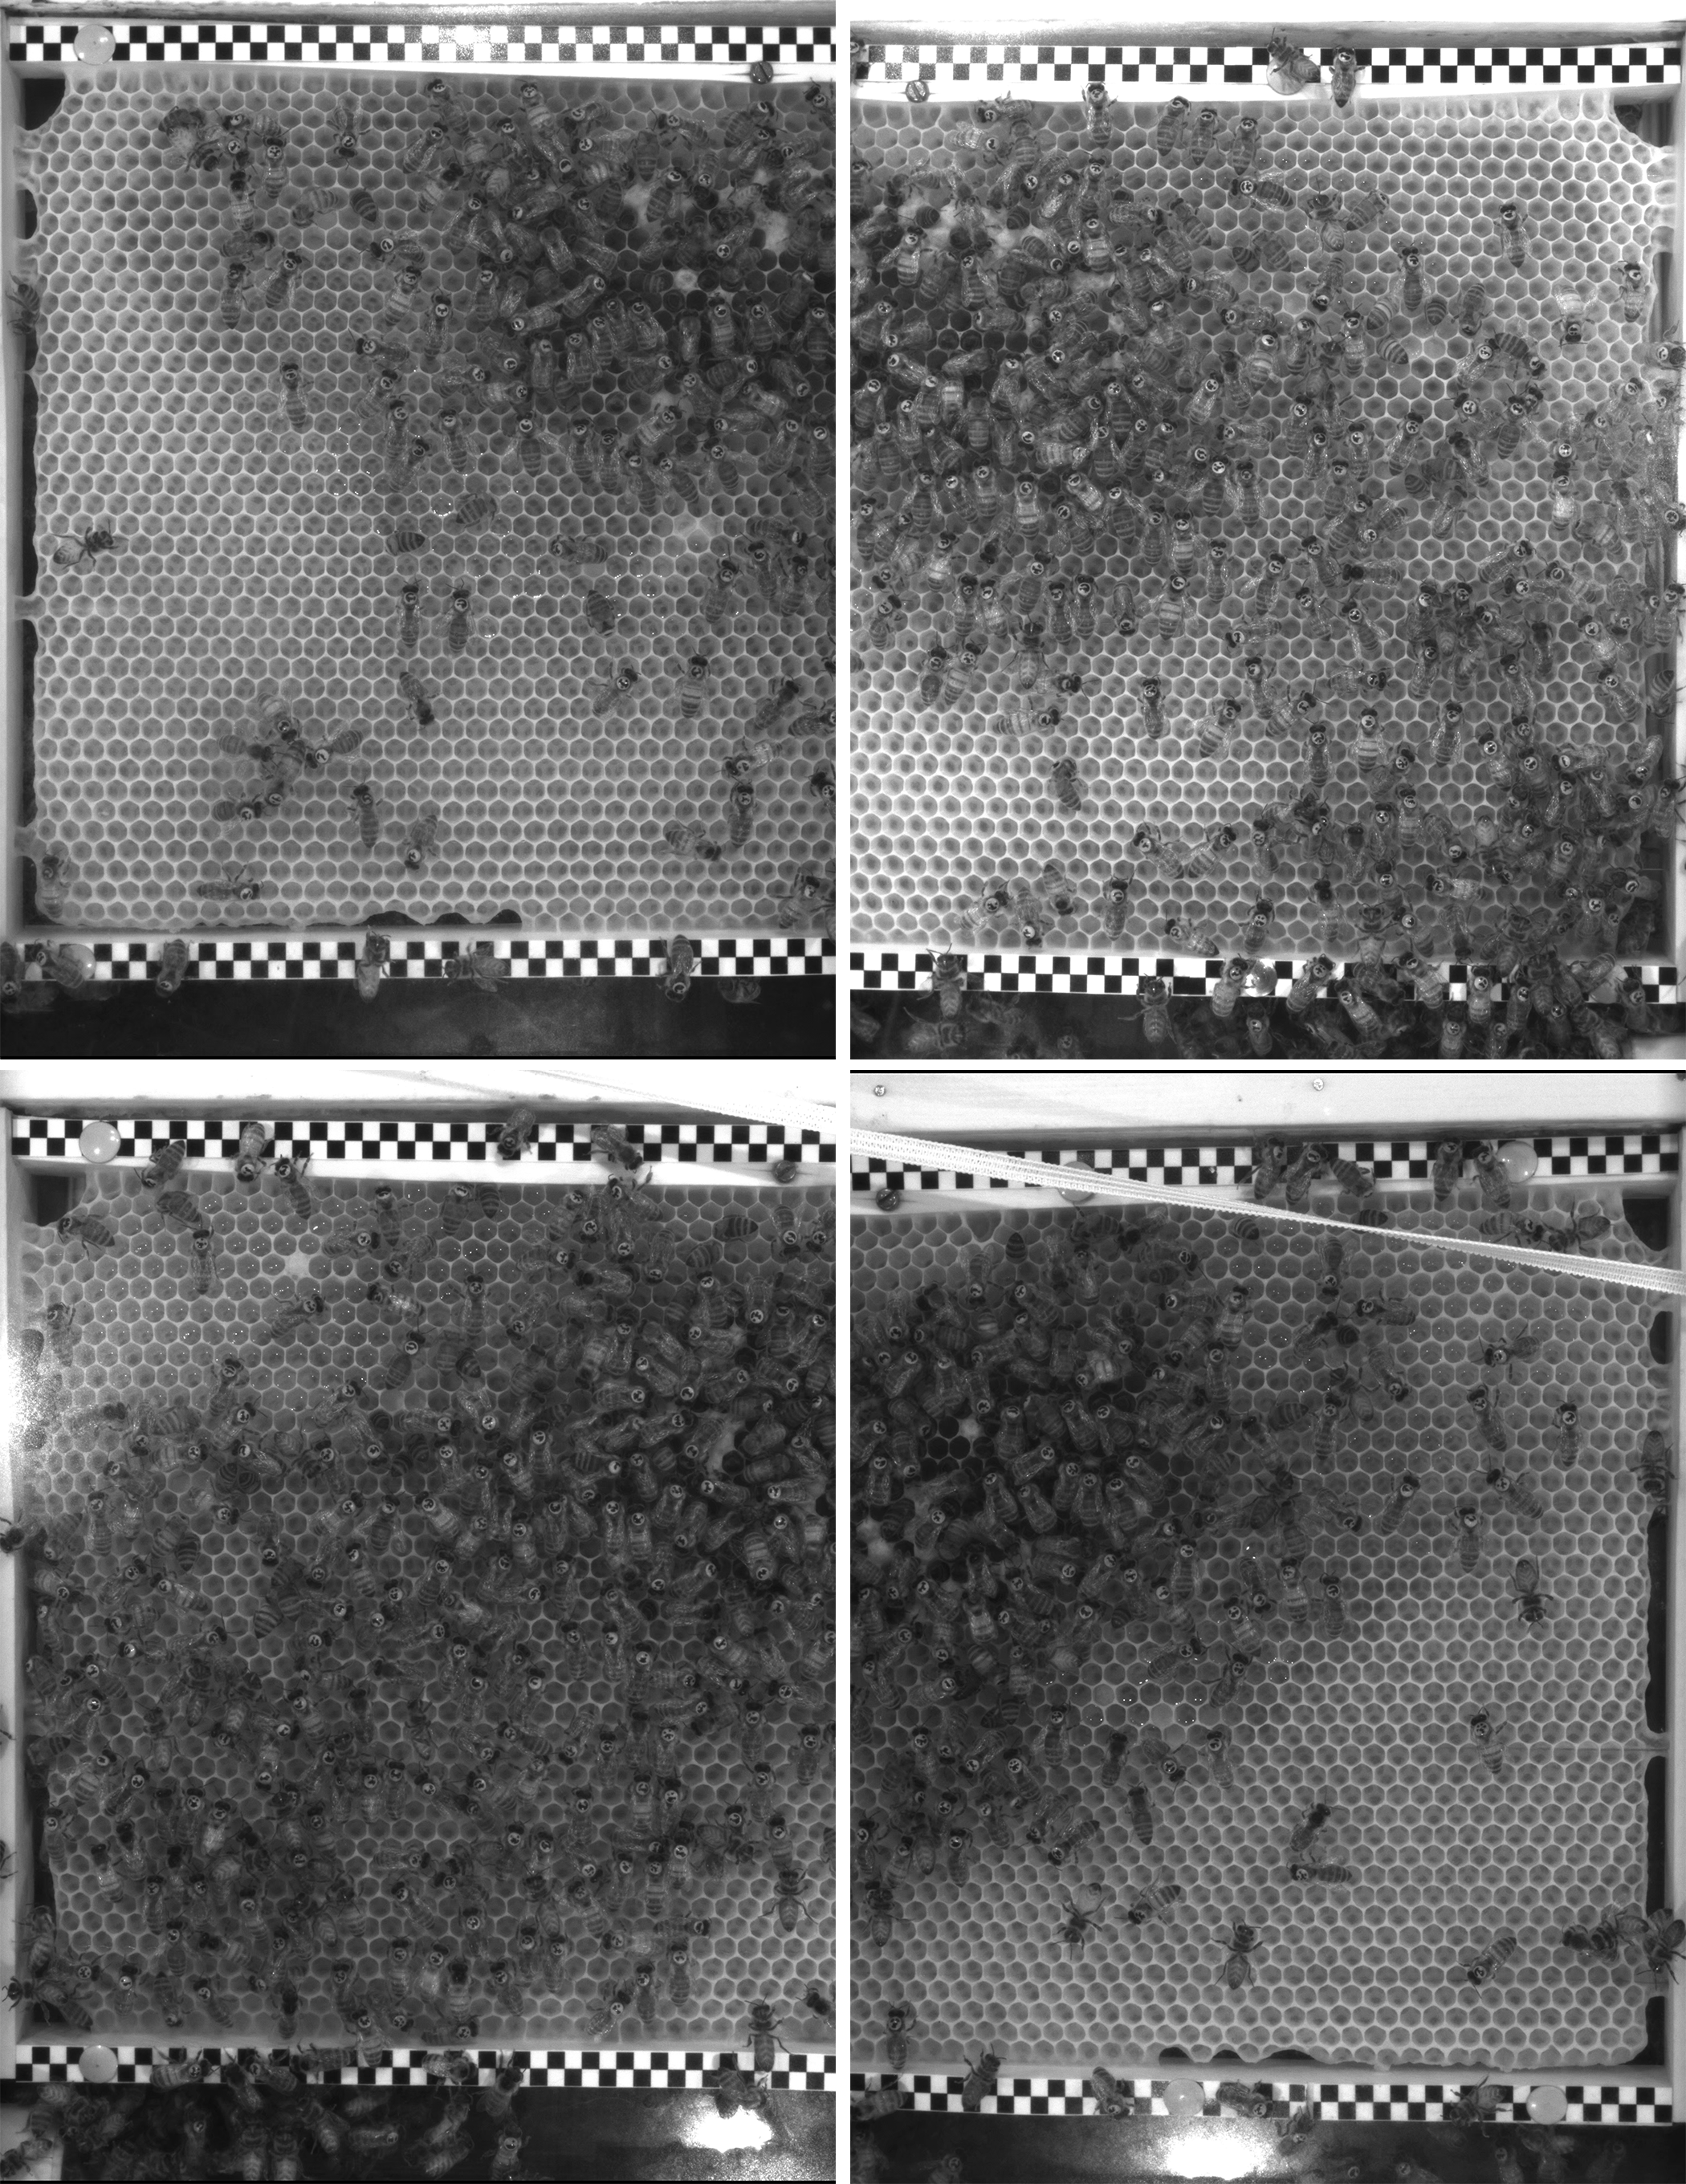
\includegraphics[width=0.8\textwidth]{Figures/beesClose}
	\caption[Images for each camera]{\textbf{Images for each camera} Top: Side~A, bottom: side~B [TODO: combine or closer to the image with camera setup]}
	\label{fig:veryclose}
\end{figure}

\begin{figure}[htb]
	\centering
	\includegraphics[width=1.0\textwidth]{Figures/tagging_period}
	\caption[Tagging frequency]{Tagging frequency: The bees were primarily tagged during the week. On average 48 bees were tagged each day, considering only tagging days, the average is about 91 ($\pm50$) bees (median 118). [TODO: combine with other image]}
	\label{fig:tagging}
\end{figure}




\clearpage
%%%%%%%%%%%%%%%%%%%%%%%%%%%%%%%%%%%%%%%%%%%%%%%%%%%%%%%%%%%%%%%%%%%%%%%%%%%%%%%
%%%%%%%%%%%%%%%%%%%%%%%%%%%%%%%%%%%%%%%%%%%%%%%%%%%%%%%%%%%%%%%%%%%%%%%%%%%%%%%
\subsection{Data Scheme}
\label{subsec:datascheme}
%%%%%%%%%%%%%%%%%%%%%%%%%%%%%%%%%%%%%%%%%%%%%%%%%%%%%%%%%%%%%%%%%%%%%%%%%%%%%%%
%%%%%%%%%%%%%%%%%%%%%%%%%%%%%%%%%%%%%%%%%%%%%%%%%%%%%%%%%%%%%%%%%%%%%%%%%%%%%%%
The data is organized in so-called \emph{frame containers}.
Each frame container corresponds to one video file of a single camera and consists of about $1024$ \emph{frames}.
Each frame holds a list of bees, which were detected by the image analysis pipeline.
A bee \emph{detection} has the following attributes:

\begin{table}[!h]
\centering
\begin{tabular}{rl}
\textbf{xpos}: & $x$ coordinate of bee with respect to the image in pixel \\
\textbf{ypos}: & $y$ coordinate of bee with respect to the image in pixel \\
\textbf{decodedId}: & decoded 12-bit id \\
\end{tabular}
\end{table}

The frame container specifies the camera, which took the video. A frame is also attributed with a timestamp. The timestamps across cameras are not identical. The data can be accessed iterating on the frame level, using two a start and end timestamp, for specifying the time interval of interest. The complete data scheme can be found on GitHub\footnote{\url{https://github.com/BioroboticsLab/bb_binary/blob/master/bb_binary/bb_binary_schema.capnp}; Last accessed: 2106-02-16, 04:46PM}. 

[TODO: schema aufmalen oder weglassen?]\\



%%%%%%%%%%%%%%%%%%%%%%%%%%%%%%%%%%%%%%%%%%%%%%%%%%%%%%%%%%%%%%%%%%%%%%%%%%%%%%%
%%%%%%%%%%%%%%%%%%%%%%%%%%%%%%%%%%%%%%%%%%%%%%%%%%%%%%%%%%%%%%%%%%%%%%%%%%%%%%%
\subsection{ID Probabilities and Confidence Level}
\label{subsec:confidence}
%%%%%%%%%%%%%%%%%%%%%%%%%%%%%%%%%%%%%%%%%%%%%%%%%%%%%%%%%%%%%%%%%%%%%%%%%%%%%%%
%%%%%%%%%%%%%%%%%%%%%%%%%%%%%%%%%%%%%%%%%%%%%%%%%%%%%%%%%%%%%%%%%%%%%%%%%%%%%%%
Twelve bits can encode the identity of 4096 bees.
Each bit of the decodedId is not a one or zero, but represents a probability between $0$ and $255$, normalized to a value between one and zero. It indicates the reliability of the image analysis pipeline for that specific bit.
I define the confidence $c$ for a bit $b$, analougus to Leon~\textcite[p.~14]{leon2016}, as $c(b)=2\cdot|b-0.5|$. The confidence of an decodedId is therefore the minimum of all bit confidences.

The amount of data that remains for further processing and its correctness depends on the chosen level of confidence. Figure~\ref{fig:remainingData} shows the relationship between confidence, the amount of remaining data and the unique number of decodedIds. The higher the chosen confidence level, the less data remains. [TODO unique IDs beschreiben]

\begin{figure}
    \centering
    \begin{subfigure}[b]{0.45\textwidth}
        \includegraphics[width=\textwidth]{Figures/confVSamount}
        \caption[Remaining Detections]{Remaining Detections depending on the level of confidence.}
        \label{fig:confVSamount}
    \end{subfigure}
    \begin{subfigure}[b]{0.45\textwidth}
        \includegraphics[width=\textwidth]{Figures/confVSids}
        \caption[Unique IDs]{Number of unique IDs depending on the level of confidence.}
        \label{fig:confVSids}
    \end{subfigure}
 	\caption[Remaining data]{\textbf{Remaining data} [TODO: beide in eins und ganze breite, welcher Datensatz, wie viele IDs waren vergeben, 100 Ids entspricht 4096]}
 	\label{fig:remainingData}
 \end{figure}   


%%%%%%%%%%%%%%%%%%%%%%%%%%%%%%%%%%%%%%%%%%%%%%%%%%%%%%%%%%%%%%%%%%%%%%%%%%%%%%%
%%%%%%%%%%%%%%%%%%%%%%%%%%%%%%%%%%%%%%%%%%%%%%%%%%%%%%%%%%%%%%%%%%%%%%%%%%%%%%%
\subsection{Time Series of Bees and Bee Pairs}
\label{subsec:tracking}
%%%%%%%%%%%%%%%%%%%%%%%%%%%%%%%%%%%%%%%%%%%%%%%%%%%%%%%%%%%%%%%%%%%%%%%%%%%%%%%
%%%%%%%%%%%%%%%%%%%%%%%%%%%%%%%%%%%%%%%%%%%%%%%%%%%%%%%%%%%%%%%%%%%%%%%%%%%%%%%

The dataset (a sequence of frames containing bee detections), is transformed to binary \emph{bee time series}, depicted in figure~\ref{fig:structure} (left and middle). A time series of a bee is a sequence of zeros and ones indicating the absence and presence of a bee over a specified time interval. 
I examined the effect the level of confidence has on the bee time serie.
As expected, with an increasing confidence level the average gap length decreases and the overall number of gaps increases (~\ref{fig:gaps}).

The number of gaps those bee time series have, is important, because in a later step I want to extract pairs of close bees, who are present at the very same time. I call those \emph{pair time series}, as shown in figure~\ref{fig:structure} (right). So a lot of gaps in bee time series, could lead to a lot of gaps in the pair time series.

\begin{figure}[htb]
	\centering
	\includegraphics[width=1.0\textwidth]{Figures/structure}
	\caption[Structure of Dataset]{\textbf{Left:} original dataset - bb\_binary data containing frames and detections; \textbf{Middle:} transformation to time series - zero indicating absence of the bee, one indicating presence of the bee; \textbf{Right:} transformation to bee pairs - zero indicating eighter one or both bees are not present at the same time or not close to each other, one indicating bees are present at the same time and nearby. [Definitiv kleiner! platzverschwendung]}
	\label{fig:structure}
\end{figure}

\begin{figure}
	\centering
	\begin{subfigure}[b]{0.45\textwidth}
		\includegraphics[width=\textwidth]{Figures/gaplen}
		\caption[Length of Gaps]{Length of Gaps depending on the level of confidence.}
		\label{fig:gaplen}
	\end{subfigure}
	\begin{subfigure}[b]{0.45\textwidth}
		\includegraphics[width=\textwidth]{Figures/numgaps}
		\caption[Number of Gaps]{Number of Gaps depending on the level of confidence.}
		\label{fig:numgaps}
	\end{subfigure}
	\caption[Influence of Confidence Level on Gaps]{Influence of the confidence level of the length of gaps and number of gaps: With an increasing level of confidence the average gap length decreases and the number of gaps per bee series increases. (Dataset: 26.07.2016, 16:00-16:05)}
	\label{fig:gaps}
\end{figure}

\clearpage
%%%%%%%%%%%%%%%%%%%%%%%%%%%%%%%%%%%%%%%%%%%%%%%%%%%%%%%%%%%%%%%%%%%%%%%%%%%%%%%
%%%%%%%%%%%%%%%%%%%%%%%%%%%%%%%%%%%%%%%%%%%%%%%%%%%%%%%%%%%%%%%%%%%%%%%%%%%%%%%
\section{Data Quality and the Detection Frequency Filter}
\label{subsec:quality}
%%%%%%%%%%%%%%%%%%%%%%%%%%%%%%%%%%%%%%%%%%%%%%%%%%%%%%%%%%%%%%%%%%%%%%%%%%%%%%%
%%%%%%%%%%%%%%%%%%%%%%%%%%%%%%%%%%%%%%%%%%%%%%%%%%%%%%%%%%%%%%%%%%%%%%%%%%%%%%%

The quality of the data could be indirectly checked using the age information of bees. On 26.07.2016, about half of the bee tags ($2014$ of $4096$) were assigned to a bee. This day was chosen to determine the effects of the confidence level on data quality.
At first, for each detection the age of that bee was calculated, a negative age was counted as a wrong detection. I assumed that the number of wrong detections indicated by negative age also occured in the positive half, but remained unseen, therefore I doubled the error. Secondly, the number of wrong unique IDs is also determinde using the age test. Figure~\ref{fig:quality} shows that even though the number of wrong detections
decreases steadily with an increasing confidence level, but the number of wrong IDs only starts to decrease with a very high level.

Even with an confidence level of $100\%$, $30.2\%$ of the unique IDs are wrong (have a negative age), corresponding to only $2.5\%$ of detections. Therefore wrong IDs need to be filtered out anyway (independent of the confidence value), to obtain a more reliable dataset. A good indicator is the detection frequency of IDs. IDs with a negative age are on average less detected than IDs with a positive age.

\begin{figure}
	\centering
	\begin{subfigure}[b]{0.45\textwidth}
		\includegraphics[width=\textwidth]{Figures/confVSdetquality}
		\caption[Wrong Detections]{Wrong detections in relation to the level of confidence.}
		\label{fig:confVSdetquality}
	\end{subfigure}
	\begin{subfigure}[b]{0.45\textwidth}
		\includegraphics[width=\textwidth]{Figures/confVSidsquality}
		\caption[Unique IDs]{Number of wrong IDs depending on the level of confidence.}
		\label{fig:confVSidsquality}
	\end{subfigure}
	\caption[Data Quality]{The number of wrong detections decreases with an increasing level of confidence. In contrast, the number of false IDS becomes noticeably less only with a very high confidence level. The amount of remaining data decreases with an increasing confidence level. The number of unique IDs behave similar. (Dataset: 26.07.2016, 16:00-16:05) (Dataset: 26.07.2016, 16:00-16:05)}
	\label{fig:quality}
\end{figure}

IDs who definately exists, but their age can to be determinded are excluded from the analysis completely. These are bees, who were tagged later~($n=10$)\footnote{id= [2,
	74,
	2045,
	3172,
	3764,
	3796,
	3827,
	3836,
	3844,
	3940]} and IDs whos detection frequency is absurd high but there age is unknown~($n=7$)\footnote{id=[has changed! 
	17,
	168,
	801,
	888,
	2045,
	2357,
	2607]}

For each analysis day the number of detections per ID is obtained, excluding the mentioned IDs above. The frequency distribution tells that, IDs with a negative age are detected less often ($704$ frames $\pm 65$)  than bees with a positive age ($36.603$ frames $\pm 2.345$). The cutoff is 99\% of the negative IDs distribution. All IDs with a detection frequency below $4737 \pm 644$ frames are discarded. A list with possible (valid) IDs is kept for each day. Using this list, faulty detections can be filtered out beforehand.


For further analysis I use the following days: 14.08.2016, 17.08.2016, 20.08.2016, 02.09.2016 with a confidence level of $95\%$. This period is chose because of XY.

Because bee time series contain a lot of short gaps (mean = 3, 95\% confidence), the inferring of edges (bees who are close to each other at the same time), should be not that strict, or at least variable. This has to be taken into acoount, when looking at spatialy close bees.






\clearpage
\section{Inferring Networks}

The following part describes the pipeline for generating spatial proximity networks out of honey bee tracking data. A node in the network is a bee. They are distinguished by IDs. Only bees are in the network who interact at least once with another bee.

undirected and weighted, aggregated networks\\

Two bees are associated (spatially close to each other), if their distance is minor to a \emph{maximum distance}. As everything is very close in a bee hive this value is hard to choose. Only this criteria is very week, meaning having a resolution of three frames per seconds results in interactions which could only last for $0.33$ seconds. So an additional parameter the \emph{minimum contact duration} is introduced, it is the minimum time they have to spend at least nearby to be called associated.

Taking the fragmentation of tracks into account, it is obvious that two bees could be nearby but not at the very same time, but slightly shifted. So the minimum contact duration would be too errow prone. To overcome this issue one could correct the bee tracks, by filling gaps of varius sizes and interpolating the position of that bee accordingly. This is rather time consuming for this amount of tracking data (TODO: naja so doll auch nicht, scipy.ndimage.morphology.binary\_dilation) and also considering, that the tracking data is going to be improved in the future, then manipulating the raw data seems senseless. I rather perform a gap filling (maybe similar to binary dilation) on the time series of pairs, but not on the bee tracks, because this is independent of the input data.

Edges are attributed with two parameters. The first one is the frequency of contacts, so how often they share a close position. The second parameter is the total duration of contact, how many time frames in total they spend close by.

\subsection{Network Pipeline}

The network pipeline takes as input a path to the bb-binary data and outputs a graph in graphML file format. The pipeline takes the following parameters:

\begin{itemize}
\item path to data
\item confidence in percent
\item gap size in frames - this is used to corret the time series of bee pairs
\item maximum distance in px - define what close means (spatial proximity)
\item minimum contact duration in frames - how many frames bees need to spend nearby
\item cutoff in percent - IDs with a number of total detections below X percent of the mean frequency are discarded 
\item start timestamp - start of network slice
\item window size in minutes - size of time window for aggregating the network
\item number of used CPUs for parallelization
\item year - calculate IDs and set camera setup for 2015 or 2016
\end{itemize}

The pipeline is parallelized on frame level, that means, each process gets a portion (frames for a timeinterval of five minutes) of the data and extracts interactions/edges. The main process adds everything up and creates a network.
The steps are the following:

\begin{enumerate}
\item \textbf{Filter detections by confidence}\\
For each of the four camera the detections are filtered by the confidence level.

\item \textbf{Simple stitching}\\
Each side of the hive consists of two cameras. 	The $x$-coordinates of each detection (of the right	cameras) is moved further to the right, also adding an offset of $2\times \texttt{maximum distance}$. So the left and the right detection of each side of the hive are move into one reference system.

\item \textbf{Syncronize Cameras}\\
For each side of the hive the cameras need to be syncronized. In the normal case the difference between consecutive frames should be about $0.332$~seconds, due to technical problem this value can be lower ($0.003$ ) and higher ($2.932$) at certain times. Cameras 3 and 2 and cameras 1 and 0 are matched, frames without a match are dropped (shorter number of frames, matchen, threshold $0.33/2$, minimum).

\item \textbf{Discard Detections with certain IDs}\\
All detections whos ID is in a list are keept, other detections are discarded. (see frequency filter)

\item \textbf{Extract close pairs}\\
For each side of the hive, all close pairs according to the maximum distance parameter are calculated and then joined together.

\item \textbf{Generate time series of bee pairs}\\
The data structure (frames and detection) is transformed to time series of bee pairs.

\item \textbf{Correct pair time series.}\\
The time series of bees are corrected by filling in the gaps of length \texttt{gap size}.

\item \textbf{Extract edges}\\
The edges and its attributes (frequency and duration) are extracted from the time series of bees using the minimum contact duration parameter. A sequence of at least X ones counts as one interaction. The frequency of those series adn the total duration (number of ones) are the attributes.


\end{enumerate}

\subsection{Pipeline Parameters}
For performing the network analysis, I chose the pipeline parameters as follows:

\begin{description}
\item[Confidence] As explained in section\ref{subsec:confidence}, the confidence is set to $95\%$.

\item[Maximum Distance] I chose the length of a bee body, according to \textcite{baracchi2014socio}, as the maximum distance between two bees (figure~\ref{fig:radius}). The average bee length of $212$px ($\pm 16$px)  was determinded by manually measuring the length of all bees ($n=337$) in four images (one for each camera, 21.07.2016, 03:00PM) using the tool ImageJ\footnote{\url{http://imagej.net/Welcome}; Last accessed: 22.02.2016}.

\item[Gap Size] The gap size is set to two frames. This value corresponds to the median gap length in the time series of pairs ($\texttt{mode}=1$, $\texttt{mean}=27$). [TODO: what dataset was used (95\% confidence, XXX\% cutOff, XXXpx maximal distance, date, camera)]

\item[Minimum Contact Duration] This is set to three frames (one second). This corresponds to~\textcite{mersch2013tracking}, they as well exclude interactions below one second. Looking at the frequency distribution of chains of ones ($1$, $11$, $111$, and so on) of the pair time series (after filling the gaps), then: $\texttt{mode}=1$, $\texttt{median}=2$ and $\texttt{mean}=4$. Three frames corresponds to $57\%$ of all chains, this seem to be reasonable. [TODO: what dataset was used (95\% confidence, XXX\% cutOff, XXXpx maximal distance, date, camera)]

\end{description}

\begin{figure}[b]
	\centering
	\begin{subfigure}[b]{0.45\textwidth}
		\centering
		\includegraphics[width=\textwidth]{Figures/radius}
		\caption[Contact Radius]{Contact Radius}
		\label{fig:radius}
	\end{subfigure}
	~ %add desired spacing between images, e. g. ~, \quad, \qquad, \hfill etc. 
	%(or a blank line to force the subfigure onto a new line)
	\begin{subfigure}[b]{0.45\textwidth}
		\includegraphics[width=\textwidth]{Figures/sizeTagBee}
		\caption[Bee and Tag Size]{Bee Length}
		\label{fig:size}
	\end{subfigure}
	\caption{Distance Between Bees: A length of a bee is chosen as the maximal  distance between bees.}
	\label{fig:contactRadius}
\end{figure}

The networks are not thresholded (according to~\cite{farine2015constructing}).

\section{Static and Temporal Analysis}

Despite the possibility of generating networks of different granularity (resolution is minutes), here for further analysis daily networks (10h, two hours after sunrise until zwo hours before sunset) are aggregated.


\textcite{wey2008social}

\subsection{Static Network Analysis}
The following network properties were analysed for a static day and hour network.\\
TODO: list of properties. (similar to what others have done)
nodes, edges, density, diameter\\


\subsection{Temporal Analysis}
three day networks (2 days gap)\\
one network 2 weeks later\\

\subsection{Community Detection}
I tested all community detection algorithms implemented in python, to find an algorithm, which works well for my case of animal social networks. The three most common python libraries for network analysis were reviewed: NetworkX\footnote{\url{https://networkx.github.io/}; Last accessed: 16.03.2016, 6:36~p.m.}, igraph\footnote{\url{http://igraph.org/python/}; Last accessed: 16.03.2016, 6:38~p.m.}, and graph-tool\footnote{\url{https://graph-tool.skewed.de/}; Last accessed: 16:03.2016, 6:39~p.m.})

The algorithm needs to fulfill the following criteria:

\begin{itemize}
\item Support for large and very dense networks ($N>1000$, $D>50~\%$)
\item Support weighted edges
\item Fast runtime
\end{itemize}

Table~\ref{tab:algos} gives an overview about the twelve algorithms reviewed. Five algorithms did not terminate after 15~minutes and were therefore excluded from further investigations. Infomap and label propagation tend to partition all nodes into a single community, this is known especially in dense graphs~\cite{yang2016comparative, fortunato2010community}.
The Louvain algorithm is the same as multilevel, but takes longer producing almost the same communities and therefore was also excluded. Walktrap was tested for different step size parameters, as suggested in~\cite{pons2005computing}, the communities remained almost the same (only a few nodes switched communities). 

I had a closer look at fastgreedy, leading eigenvector, multilevel, and walktrap regarding the number of detected communities and community size for all three networks. Table~\ref{tab:algos4} shows the results. All algorithms found at least two communities. Except for leading eigenvector, there is a tendency that a third community exists.
I decided to use two algorithms for community detection: leading eigenvector and walktrap. \textcite{farine2015constructing} explains that leading eigenvector is often used with animal social networks and works well. Walktrap is chosen for also  examining the possible third community.

There are comparative analysis of community detection algorithms, e.g.~\cite{yang2016comparative, harenberg2014community}. They seem to be promising, but assume eighter a power law degree distribution or evaluate networks with a low density, which is not applicable here.

\begin{table}[htbp]
\small
\caption[Compairing community detection algorithms]{\textbf{Comparing community detection algorithms} Comparison of algorithms implemented in python. Criteria are the support of weighted links, runtime and number of communities. A runtime indicated by ``$-$'' means no termination after 15~minutes.\\
}
\label{tab:algos}

\begin{tabularx}{\textwidth}{lcccccccccccc}
\toprule
	 {} &
	 \rotatebox{90}{\textbf{Fastgreedy$^1$}} &
	 \rotatebox{90}{\textbf{Leading eigenvector$^1$}} &
	 \rotatebox{90}{Louvain$^2$} &
	 \rotatebox{90}{\textbf{Multilevel$^1$}} &
	 \rotatebox{90}{\textbf{Walktrap$^1$}} &
	 
	 \rotatebox{90}{Infomap$^1$} &
	 \rotatebox{90}{Label propagation$^1$} &
	 
	 \rotatebox{90}{Edge betweenness$^1$} &
	 \rotatebox{90}{K-clique communities$^2$\thinspace} &
	 \rotatebox{90}{Optimal modularity$^1$} &
	 \rotatebox{90}{Spinglass$^1$} &
	 \rotatebox{90}{Statistical inference$^3$} \\ \midrule
	 
	 
	 
	 Link weights & $\times$ & $\times$ & $\times$ & $\times$ & $\times$ & $\times$ & $\times$ & & $\times$ & $\times$ & $\times$ \\ \midrule
	 Runtime in sec & ~$3.6$ & ~$6.3$ & $11.7$ & ~$0.7$ & $19.4$ & $13.2$ & ~$0.2$ & $-$ & $-$ & $-$ & $-$ & $-$ \\ \midrule
	 Communities & $3$ & $2$ & $2$ & $3$ & $2$ & $1$ & $1$ & $-$ & $-$ & $-$ & $-$ & $-$ \\ \midrule
	 Size & 473 & 488 & 469 & 462 & 490 & 922 &  922 &  &  &  &  &  \\
	  & 434 & 434 & 453 & 427 & 431 &  &  &  &  &  &  &  \\
	  & 15 &  &  & 33 & (1) &  &  &  &  &  &  &  \\
	 \bottomrule
	 
\end{tabularx}
\begin{flushright}
\footnotesize{
$^1$ igraph, $^2$ NetworkX, $^3$ graph-tool\\
}
\end{flushright}

\end{table}

% \hdashline
% \midrule
% \bottomrule
\begin{table}[htbp]
\small
\centering
\caption[Number of community members per algorithm and snapshot]{\textbf{Number of community members per algorithm and snapshot} Four algorithms were tested and compared regarding the number of detected communities and the size of the communities.\\
}
\label{tab:algos4}

\begin{tabular}{lcccc}
\toprule
	 {} &
	 \rotatebox{90}{Fastgreedy} &
	 \rotatebox{90}{\textbf{Leading eigenvector}} &
	 \rotatebox{90}{Multilevel} &
	 \rotatebox{90}{\textbf{Walktrap}} \\ \midrule
	 
	  Snapshot 1
	  & 473 & 488 & 462 & 490 \\
	  & 434 & 434 & 427 & 431 \\
	  & 15 &   & 33 & (1) \\ \midrule
	  Snapshot 2
	  & 504 & 503 & 481 & 372 \\
	  & 467 & 475 & 439 & 311 \\
	  & 7 &   &  58 & 294 \\
	  & & & & (1) \\ \midrule
	  Snapshot 3
	  & 534 & 537 & 505 & 310 \\
	  & 388 & 385 & 415 & 390 \\
	  &  &   &  (2) & 231 \\
	 \bottomrule
\end{tabular}
\end{table}

% \hdashline
% \midrule
% \bottomrule

\section{Attributed Data and Hypothesis Testing}
Hypothesis\\
(1) Communities reflect groups of bees working in different areas of the hive and\\
(2) Communities reflect different age groups\\

The data which was used to test the hypothesis (1) is saved in a sqlite database for faster access, because using bb\_binary (parsing the data over and over again) was to slow. For testing if lists of positions (spatial ditribution) are different the test XY was used [TODO: what to use here]

For hypothesis (2) the data is stored as a csv file of birth dates of each bee. For testing if age goups are different the Kolmogorov Smirnov Test was used.

\section{Implementation, Runtime and Complexity}
For implementing the network pipeline python, with pandas and numpy, are used, because the bb\_binary library, for accessing the tracking, data is only available in python. The networks, in graphML format, are created using the python library \emph{NetworkX}\footnote{\url{https://networkx.github.io/} ; Last accessed: 2017-02-17, 08:07PM} in version 1.11.
iGraph for community detection\\
some bash scrips for generating multiple networks\\

bottleneck is reading bb\_binary data into pandas dataframes\\
using multithreading for distribution on frame level (a process gets X frames for processing)\\

maybe some table with how long nees what with how many cores (hom much RAM and so on)\\